\mode<presentation>{
\begin{frame} 
    \begin{center} \huge
        From Non-parametric classification\\
        to RBF-Networks
    \end{center}
\end{frame}
}

\section{Non-parametric classification}

\subsection{The setting}

\begin{frame}\frametitle{\subsecname~for M-way classification}

\mode<article>{
Specifying the data and model for a multi-class classification with $M$ classes (i.e. $M$-way classification)
}

\begin{itemize}
	\item[]\underline{Data}:
	\begin{equation*}
	\Big\{ \left(\vec x^{(\alpha)}, \vec y^{(\alpha)}_{T} \right) \Big\}_{\alpha=1}^{p}\,
	\end{equation*}

	where $\vec y_T^{(\alpha)} \in \{0, 1\}^M$ with $\sum_{c=1}^{M} (y_{T})_c = 1$ (one-hot encoding of class labels)\\

	\pause

	\item[]\underline{Model}:
	\begin{equation*}
	\vec y(\vec x) \in \R^M 
	\end{equation*}
	with $\sum_{c=1}^{M} y_c(\vec x) = 1$ and $y_c(\vec x)\,\ge\,0\; \forall\,c$\\[2mm]
	
	Predictions $\vec y(\vec x)$ can be used to give
	\begin{itemize}
	\item probabilities of the predicted class (e.g. $y_5(\vec x) = 0.75\; \leadsto$ class ``5'' with 75\% probability.
	\item hard decisions:
    \begin{equation}
    \argmax_{c=1,\ldots,M}\;y_c(\vec x)
    \end{equation}
	\end{itemize}

\end{itemize}

\end{frame}

\subsection{k nearest neighbor classifier}

\begin{frame}\frametitle{\subsecname}
Prediction follows an \emph{electoral committee}; the majority vote of the $k$ nearest neighbors around the query point.

\begin{figure}[h]
	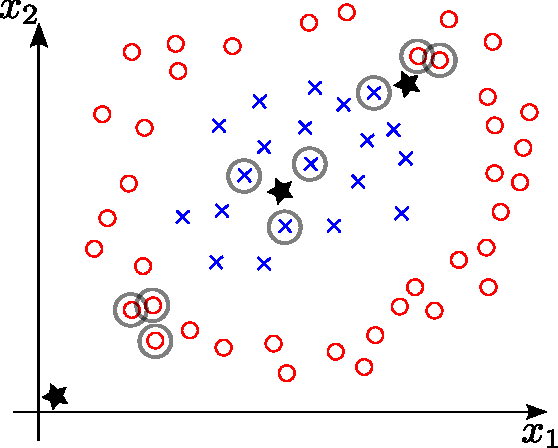
\includegraphics[width=0.3\textwidth]{img/knn}
	\mode<article>{
	\caption{$k$NN with $k=3$}
	}
\end{figure}

Let $k$NN$(\vec x)$ be the indices $\{\beta_1, \beta_2,\ldots,\beta_k\}$ of the $k$ data points closest to $\vec x$ w.r.t. Euclidean norm:

\begin{equation}
\beta_j = 
\argmin_{\substack{\kern-2ex \alpha \in \{1,\ldots,p\} \,\textbackslash\\ \{\beta_{1},\ldots,\beta_{j-1}\}}}
\lVert \vec x^{(\alpha)} \kern-.8ex - \vec x\rVert_{2}
\end{equation}

\end{frame}

\subsubsection{For multi-class classification}

\begin{frame}\frametitle{\subsubsecname}

For multi-class classification the $k$NN classifier (for fixed $k~\corresponds$ hyper-parameter) is defined by:

\begin{equation}
\vec y(\vec x) = \frac{1}{k} \sum_{\beta \in k\mathrm{NN}(\vec x)} \kern-0.5ex \vec y_{T}^{(\beta)}
\label{eq:knn_classifier}
\end{equation}

$\vec y(\vec x)$ \notesonly{in \eqref{eq:knn_classifier}} is effectively an arithmetic average of the labels in the neighborhood.

\end{frame}

\begin{frame}
Example k=3, M=4

\begin{equation}
\vec y(\vec x) = \frac{1}{3}
\left\lbrack
\,
\rmat{ 1 \\ 0 \\ 0 \\ 0}\, +\,
\rmat{ 1 \\ 0 \\ 0 \\ 0} +\,
\rmat{ 0 \\ 1 \\ 0 \\ 0}\,
\right\rbrack
=
\frac{1}{3}
\rmat{ 2 \\ 1 \\ 0 \\ 0}
=
\rmat{ 2/3 \\ 1/3 \\ 0\; \\ 0\;}
\end{equation}

applying a hard decision would yield $c=1$.
    
\end{frame}

\subsubsection{the binary classification case}

\begin{frame}\frametitle{\subsubsecname}

For binary classification, we can set $M=2$ for a multi-class $k$NN classifier.

Alternatively, we can construct the $k$NN classifier \notesonly{for binary classification} using \emph{scalar} labels:

\begin{equation}
y_T \in \{0,1\}\quad \text{ and }\quad y(\vec x) \in \R
\end{equation}
with

\begin{equation}
y(\vec x) \ge\,0\,:\,
\begin{cases*}
      \;y(\vec x) & probability of class $1$ \\
      \;1-y(\vec x)     & probability of class $0$
    \end{cases*}
\end{equation}

\end{frame}

\begin{frame}

\question{What is the role of $k$ in terms of model complexity? $k = 1$ vs. $k = p$}

\mode<presentation>{

\begin{figure}[h]
	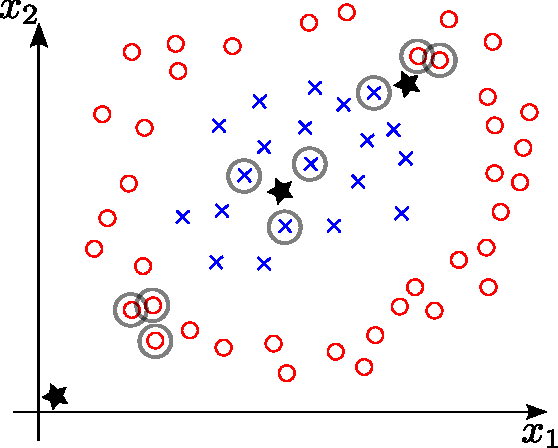
\includegraphics[width=0.4\textwidth]{img/knn}
	\mode<article>{
	\caption{$k$NN with $k=3$}
	}
\end{figure}

}

\pause

\question{How would you select the $k$ nearest neighbors for some query point $\vec x$?}

\pause

Hint: Jitter the data (or the query points) and see which choice of $k$ leads to different (more noisy) predictions.

\mode<article>{

Remarks:
\begin{enumerate}
\item The value of $k$ controls the model complexity ($k = 1 \leadsto$ over-fitting, larger $k \leadsto$ under-fitting)

\item Selecting the $k$ nearest neighbors of some point $\vec x$ can be costly but can be made more efficient using data structures such as \emph{Kdtrees})
\end{enumerate}
}

\end{frame}
